\documentclass[a4paper]{article}
\usepackage{pstricks}
\usepackage{amsmath}
\usepackage{graphicx}
\usepackage{pdfpages}
\usepackage{mathrsfs}

\setlength{\unitlength}{1.0mm}
\sloppy

\begin{document}

\title{Credit Score Cards - Notes}
\author{Michal Mackanic}
\date{December 2019}
\maketitle

\tableofcontents{}

\section{Sensitivity and Specificity}

Sensitivity and specificity are statistical measures of performance of a binary classifier.

Sensitivity, also known as true positive rate, recall or probability of detection, measures the proportion of actual positives that are correctly identified (e.g., percentage of sick people who are correctly identified as sick).

Specificity, also called true negative rate, measures the proportion of actual negatives that are correctly identified (e.g., percentage of healthy people who are incorrectly identified as sick).

\begin{equation}
\textit{sensitivity} = \frac{\textit{number of true positives}}{\textit{number of true positives} + \textit{number of false negatives}}
\end{equation}

\begin{equation}
\textit{specificity} = \frac{\textit{number of true negatives}}{\textit{number of true negatives} + \textit{number of false positives}}
\end{equation}

A highly sensitive test rarely overlooks an actual positive; a highly specific test rarely registers a positive classification for anything that is not the target of testing.

Sensitivity therefore quantifies the avoidance of false negatives and specificity does the same for false positives. For any test, there is usually a trade-off between the measures. For instance, in airport security, since testing of passengers is for potential threads to safety, scanners might be set to trigger alarm on low-risk items like belt buckles (low specificity) in order to increase the probability of identifying dangerous objects. This trade-off could presented graphically using a receiver operating characteristic (ROC) curve.

\subsection{Confusion matrix}

Consider a group with $P$ positive instances and $N$ negative instances of some condition. Four possible outcomes can be formulated in a 2x2 confusion matrix.
\begin{figure}[htp]
\centering
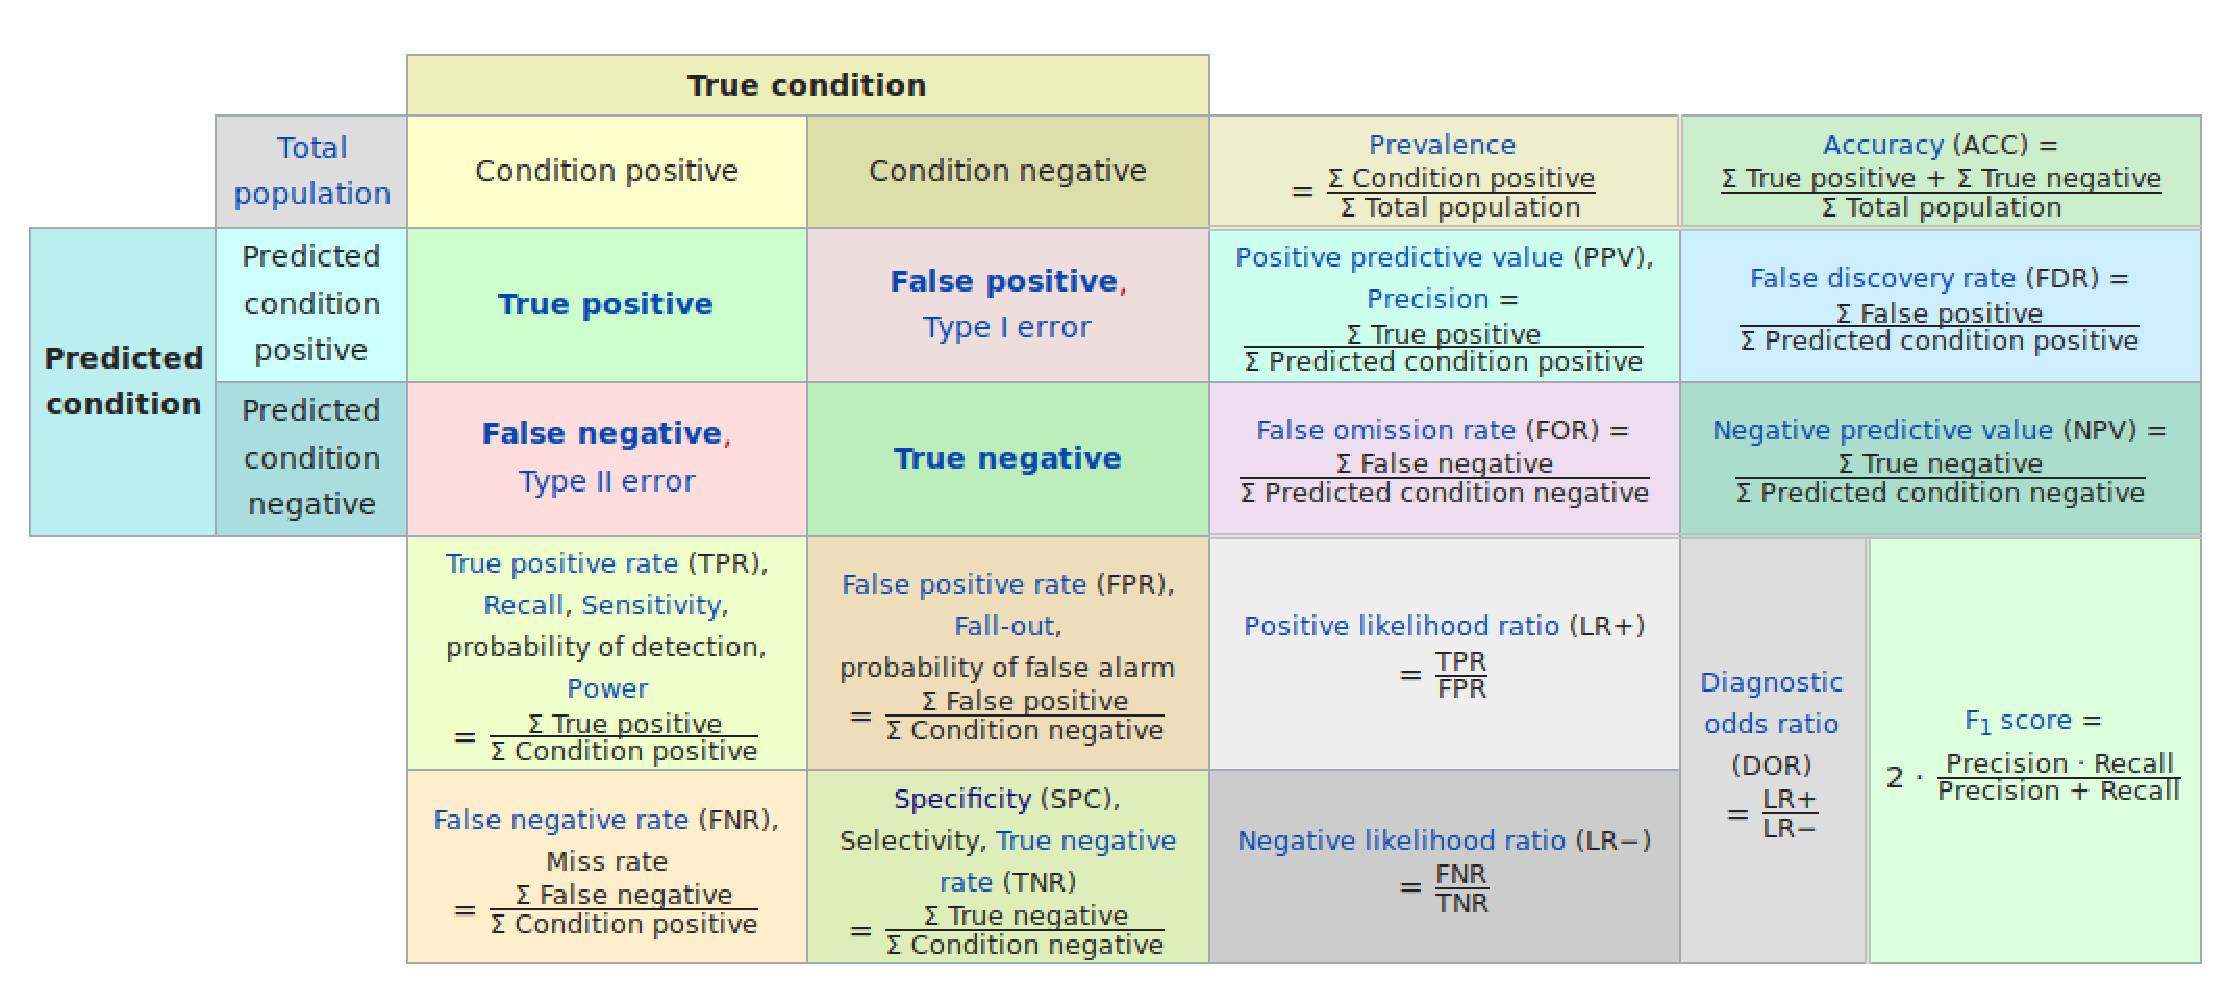
\includegraphics[scale = 0.35]{pictures/confusion_matrix.eps}
\caption{Confusion matrix}
\label{fig_conf_mtrx}
\end{figure}	

\section{Receiver operating characteristic}

A receiver operating characteristic (ROC) curve is evaluates diagnostic ability of a binary classifier.

The ROC curve plots true positive rate (TPR) against false positive rate (FPR) for various levels of the binary threshold. In machine learning the true positive rate is also known as sensitivity, recall or probability of detection. The false positive rate is then known as probability of false alarm and could be calculated as $1 - \textit{specificity}$. If probability distributions of detection and false alarm are know, the ROC curve could be generated by plotting cumulative distribution function of detection probability in the y-axis versus cumulative distribution of the false-alarm probability on x-axis.

\end{document}